\section{The product}

\subsection{Layout}
\begin{figure}
   \centering
   \includegraphics[scale=0.6]{irudiak/pantallazo.png}
   % Laster-markak gehitzeko menua
   \caption{Screenshot of the main screen}
   \label{fig:pantailazo}
\end{figure} 

In figure no. \ref{fig:pantailazo} the intended main screen is shown, taken from the working program but based on previous hand-made sketches. On the left, active downloads appear, showing graphically the progress of them, using a progress bar. On the left, the names of the downloadable files appears along with the file size. To download one of those, it is enough to click the \texttt{deskargatu} button and in case we want to refresh the list of available files, we should click \texttt{aktualizatu}.

No information about uploading appears, as there is no user interaction regarding this matter.

\subsection{Working process}
In this section, the main functionalities of the program are explained, one layer deeper that has been shown in the Methodology section. Here, in-depth schemas are in place, using mainly Sequential UML diagrams. It has to be mentioned, though, that the text in those diagrams are in Basque language, the same language the codification of the program has been made. That way it will be simpler to compare the diagrams with the code rather than translating function and object names into English just for the diagrams. But, on the contrary, all the explanations of the diagrams are done in English. Also, the bulk of the diagrams focuses on the client, because it is the part where the real work is done. As said, servers just put clients together. Not all the code is featured in the diagrams (graphical interfaces etc. have been left apart), and just the distributed nature of the application is shown.

\begin{figure}
   \centering
   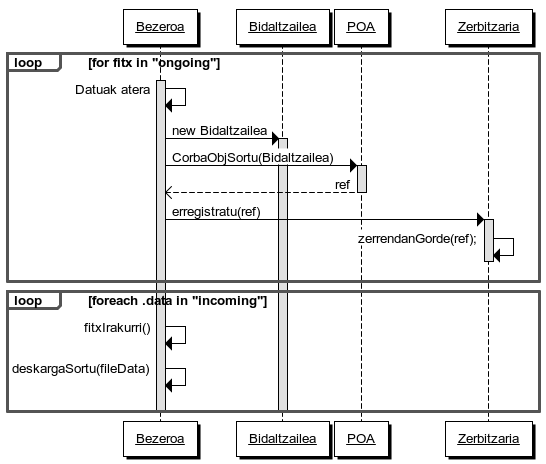
\includegraphics[scale=0.6]{irudiak/bezeroahasiera.png}
   % Laster-markak gehitzeko menua
   \caption{Start of the P2P client}
   \label{fig:hasiera}
\end{figure} 

In the figure no. \ref{fig:hasiera} it is possible to see what the client does when it is started.  First, extracts the identification data of the file (file name, hash as defined in the IDL, look section \ref{sec:met}), after creates  the \texttt{Bidaltzailea} object, whose responsibility is to upload the content the user is sharing. Finally, it creates a Corba object with it and registers it in the Server. This process is repeated with all the files in the \texttt{ongoing} directory. 

\begin{figure}
   \centering
   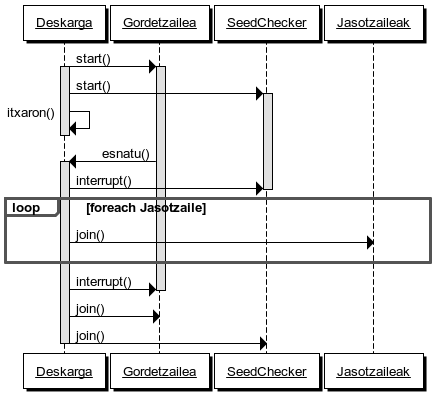
\includegraphics[scale=0.6]{irudiak/deskargenruna.png}
   % Laster-markak gehitzeko menua
   \caption{Run of the \texttt{Deskarga} thread.}
   \label{fig:deskarga}
\end{figure} 

Figure no \ref{fig:deskarga} shows the development of the download (\texttt{Deskarga}) process. Each download is initialized with one \texttt{SeedChecker} and one \texttt{Gordetzaile} object and it is the \texttt{Deskarga} object who starts the \texttt{Gordetzaile} and \texttt{SeedChecker}, and when the \texttt{Gordetzaile} tells the \texttt{Deskarga} that it is awake, that is, the download is complete; interrupts the \texttt{SeedChecker}, waits to all the \texttt{Jasotzaileak} threads (each one downloads the content from a different client), interrupts the \texttt{Gordetzailea} and waits until all the remaining threads are finished.

\begin{figure}
   \centering
   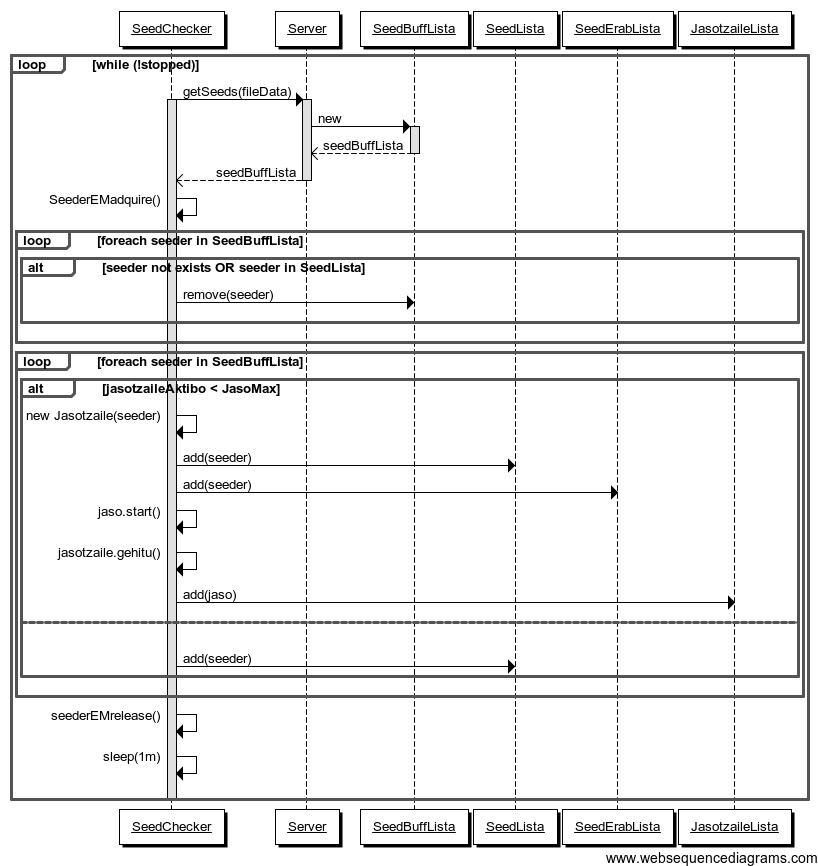
\includegraphics[scale=0.5]{irudiak/seedaktxekeatu.png}
   % Laster-markak gehitzeko menua
   \caption{Run of the \texttt{SeedChecker} thread.}
   \label{fig:seedtxeker}
\end{figure}  

The process of retrieving the seeds from the server is done by the \texttt{SeedChecker} thread (figure no. \ref{fig:seedtxeker}) and each . Starts retrieving the seeds from the server, with the data extracted from the file (see the \texttt{Datuak atera} process in figure no. \ref{fig:hasiera}). The server creates a Buffer list of the seeders and returns it to the client. The process described next is done using a mutual exclusion semaphore, to make sure that the objects mentioned are not manipulated at the same time. 

The checker checks all that the seeders actually all the seeders exist or that are not in the \texttt{SeedLista} object, because that means that a file is being downloaded from them at the moment. As shown in the diagram no. \ref{fig:deskarga} the client creates a \texttt{Bidaltzailea} for each file, which is, in fact the seeder from the file is downloaded. Thus, having a seeder in the \texttt{SeedLista} means that the client is already downloading the same content from it and therefore is removed from the buffer. 

Once the duplicated and inexistent seeders have been put away, for each seeder from the now clean buffer the system checks if the active seeder number (each active seeder has an active \texttt{Jasotzaile}) is less than the maximun one (\texttt{JasoMax}) and if it is, the \texttt{SeederChecker} registers the seeder in the \texttt{SeedLista} \texttt{SeedErabLista}. This last object is used to store the seeders that are actually in use, to prevent creating a new \texttt{Jasotzaile} with a seeder already in use. A \texttt{Jasotzaile} is created with a seeder that is in \texttt{SeedLista} but is not in \texttt{SeedErabLista}. After the creation of the Jasotzaile, the checker adds the newly created one to the \texttt{JasotzaileLista} list. But, if the active seeder number exceeds the maximun one, the new seeder is just registered in the \texttt{SeedLista} not in the \texttt{SeedErabLista}. Finally, the semaphore opens again and the process sleeps until is rerun again.

\begin{figure}
   \centering
   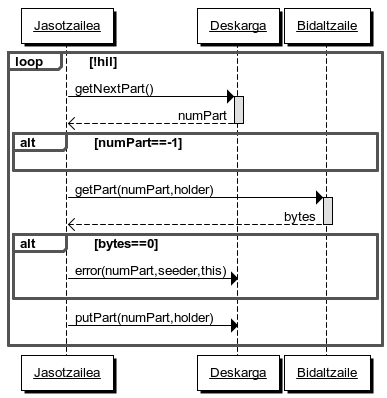
\includegraphics[scale=0.45]{irudiak/jasotzailerun.png}
   % Laster-markak gehitzeko menua
   \caption{Run of the \texttt{Jasotzailea} thread.}
   \label{fig:jasotzaile}
\end{figure}  

The next process, concerning the retrieving of files, is done by the thread \texttt{Jasotzailea}, as shown in figure no. \ref{fig:jasotzaile}. It has already been mentioned how a \texttt{Jasotzaile} is created by the \texttt{SeedChecker}. Them the newly created object asks for the number of the next downloadable part. If that number is \texttt{-1}, the thread is interrupted. If it is not, asks to the \texttt{Bidaltzaile} of the seeder the next part of the file. If the part received has a size of 0 bytes, the thread files and error and starts the loop again. Unlike the previous break, this break does not interrupt the thread, just starts the loop again. If some bytes are received, the \texttt{Jasotzailea} just forwards those to the \texttt{Deskarga} object. All this it is done if there is no exceptional error which changes the \texttt{hil} value to \texttt{true}.

\begin{figure}
   \centering
   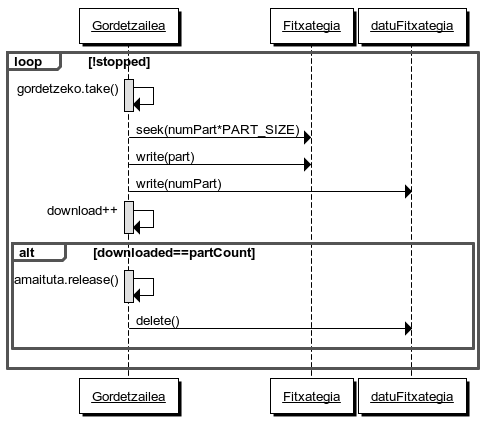
\includegraphics[scale=0.6]{irudiak/gordetzaileruna.png}
   % Laster-markak gehitzeko menua
   \caption{Run of the \texttt{Gordetzailea} thread.}
   \label{fig:gordetzailea}
\end{figure}  

The process of storing the file is controled by the \texttt{Gordetzailea} thread (shown in figure no. \ref{fig:gordetzailea}), which basically writes what has been received. All the process is regulated by a mutual exclusion semaphore, so no concurrence problems occur. The object is created with the data retrieved by the other client (see the \texttt{Datuak atera} process in figure no. \ref{fig:hasiera}). It basically writes received parts to the file (\texttt{Fitxategia}) and writes to a \begin{verbatim}.data\end{verbatim} (\texttt{datuFitxategia}) file what has been the last part downloaded, so the download can be resumed in the same place if the process is interrupted (in case the network goes down, for instance). After, if the downloaded part number is the same as the number of parts the file has, the semaphore opens, the auxiliary \begin{verbatim}.data\end{verbatim} file is erased and the \texttt{stopped} variable is set to true, so the process does not continue. If there are parts still to store, the process just repeats again.

\begin{figure}
   \centering
   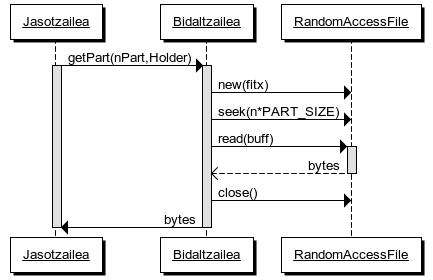
\includegraphics[scale=0.6]{irudiak/bidaltzailerun.png}
   % Laster-markak gehitzeko menua
   \caption{\texttt{Bidaltzailea} sending files method.}
   \label{fig:bidaltzailea}
\end{figure}  

The last process shown in this report (figure no.\ref{fig:bidaltzailea}), is the one that affects the sending of files. Unlike the previous ones, this process is not started with an explicit \texttt{start()} method, Corba itself executes it in a separate thread, as the reincarnation of the methods stated in the IDL file. So, when a \texttt{Jasotzailea} asks for a new part, the \texttt{Bidaltzailea} reads the bytes concerned and sends them back. The reason to use RandomAccessFiles is that the file can be read simoultaneously and can be chosen which part is read, using the \texttt{seek()} function.

With this six processes, the main functions of how our P2P program shares the files is explained, leaving secondary explanations aside.

\subsection{Program structure}
To achieve the functionalities presented in the previous section, it is necessary to go down to the code, to see how it is arranged and how different methods interact with each others. But, in this case, leaving the code apart, class diagrams are going to be shown, the last step of the unified procedure of this program. In those, methods and variables appear, ordered by the class they belong. 

\begin{figure}
   \centering
   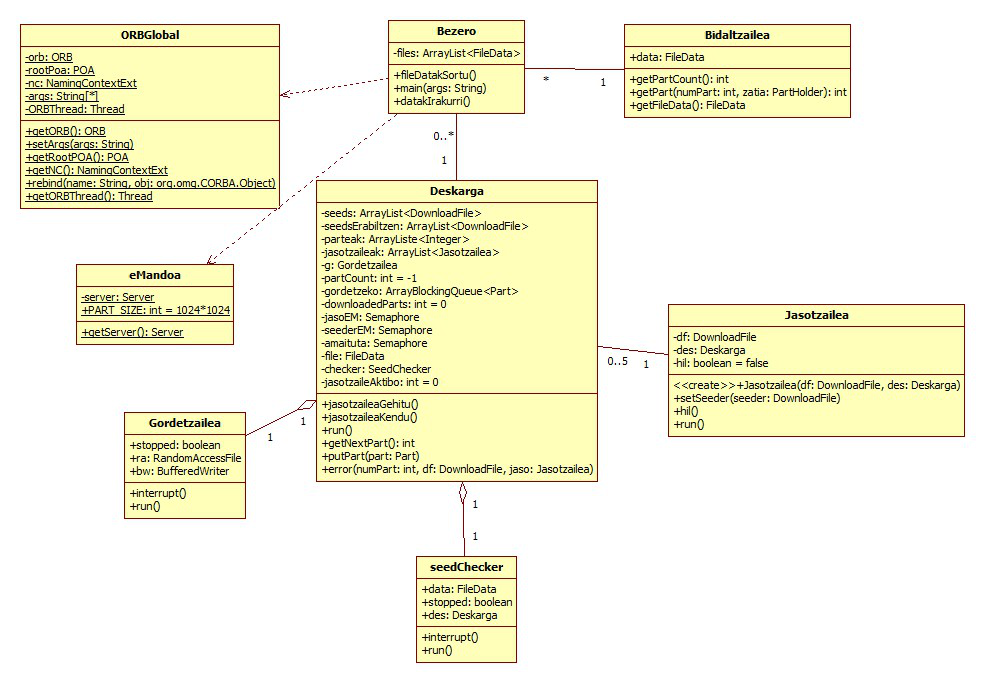
\includegraphics[scale=0.5]{irudiak/BezeroKlaseDiagrama.png}
   % Laster-markak gehitzeko menua
   \caption{Class diagram of the client}
   \label{fig:klasebezero}
\end{figure}  

\begin{figure}
   \centering
   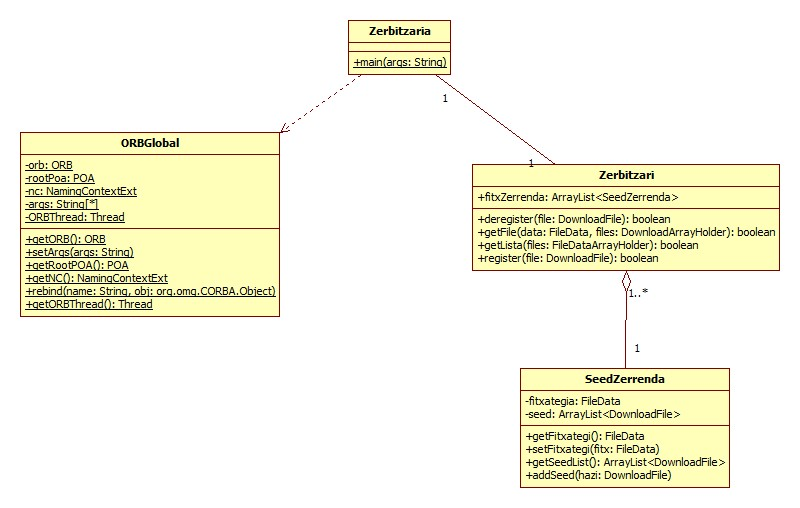
\includegraphics[scale=0.5]{irudiak/ZerbitzariKlaseDiagrama.png}
   % Laster-markak gehitzeko menua
   \caption{Class diagram of the server}
   \label{fig:klasezerbitzaria}
\end{figure}
 
In both diagrams, all the methods mentioned in the previous section appear ordered, as well as the cardinality of the relation between the classes that host them. From those clases, \texttt{Bidaltzailea} is the reincarnation of the \texttt{DownloadFile} defined in the IDL and \texttt{Zerbitzari}, the one of \texttt{server}. 